\documentclass[tikz, border=2pt]{standalone}

\usepackage{amsmath,amssymb}
\usepackage{pgfplots}
\pgfplotsset{compat=1.18}
\usepgfplotslibrary{groupplots}
\usetikzlibrary{arrows.meta}
\usepackage{xcolor}

\definecolor{utnblue}{RGB}{0, 51, 102}

\begin{document}
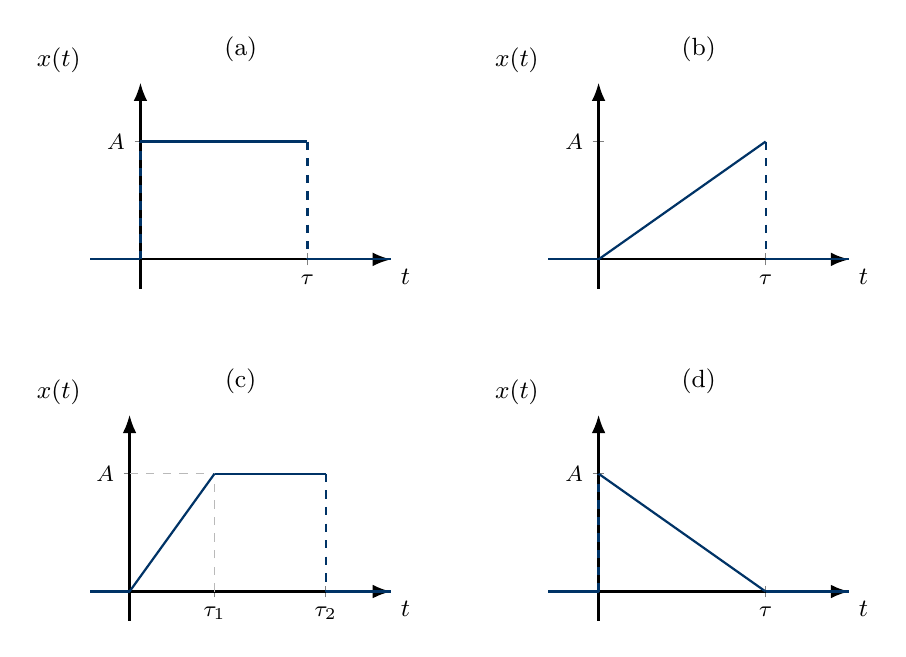
\begin{tikzpicture}[>=Latex, font=\small]

\pgfplotsset{
  every axis/.append style={
    axis lines=middle,
    axis line style={->, thick, black},
    width=5.4cm, height=4.2cm,
    xlabel={$t$}, ylabel={$x(t)$},
    xlabel style={anchor=north west},
    ylabel style={rotate=0, anchor=south east, at={(axis description cs:0,1)}},
    ymin=-0.25, ymax=1.5,
    ytick={1}, yticklabels={$A$},
    yticklabel style={font=\footnotesize},
    xticklabel style={font=\footnotesize},
    title style={yshift=-2pt},
    clip=false,
  },
  sig/.style={utnblue, thick},        % trazo de la señal
  jump/.style={utnblue, thick, dashed}, % discontinuidad (salto vertical)
  guia/.style={gray!55, thin, dashed},  % líneas guía de coordenadas
}

\begin{groupplot}[
  group style={group size=2 by 2, horizontal sep=2cm, vertical sep=1.6cm},
]
  % ===== (a) Pulso rectangular =====
  \nextgroupplot[xmin=-0.6, xmax=3, xtick={2}, xticklabels={$\tau$}, title={(a)}]
    \addplot[sig] coordinates {(-0.6,0) (0,0)};
    \addplot[sig] coordinates {(0,1) (2,1)};
    \addplot[sig] coordinates {(2,0) (3,0)};
    \addplot[jump] coordinates {(0,0) (0,1)};
    \addplot[jump] coordinates {(2,1) (2,0)};

  % ===== (b) Rampa limitada =====
  \nextgroupplot[xmin=-0.6, xmax=3, xtick={2}, xticklabels={$\tau$}, title={(b)}]
    \addplot[sig] coordinates {(-0.6,0) (0,0)};
    \addplot[sig] coordinates {(0,0) (2,1)};
    \addplot[sig] coordinates {(2,0) (3,0)};
    \addplot[jump] coordinates {(2,1) (2,0)};

  % ===== (c) Trapezoidal =====
  \nextgroupplot[xmin=-0.6, xmax=4, xtick={1.3,3}, xticklabels={$\tau_1$,$\tau_2$}, title={(c)}]
    \addplot[guia] coordinates {(0,1) (3,1)};
    \addplot[guia] coordinates {(1.3,0) (1.3,1)};
    \addplot[sig] coordinates {(-0.6,0) (0,0)};
    \addplot[sig] coordinates {(0,0) (1.3,1)};
    \addplot[sig] coordinates {(1.3,1) (3,1)};
    \addplot[sig] coordinates {(3,0) (4,0)};
    \addplot[jump] coordinates {(3,1) (3,0)};

  % ===== (d) Rampa decreciente =====
  \nextgroupplot[xmin=-0.6, xmax=3, xtick={2}, xticklabels={$\tau$}, title={(d)}]
    \addplot[sig] coordinates {(-0.6,0) (0,0)};
    \addplot[sig] coordinates {(0,1) (2,0)};
    \addplot[sig] coordinates {(2,0) (3,0)};
    \addplot[jump] coordinates {(0,0) (0,1)};
\end{groupplot}
\end{tikzpicture}
\end{document}
